\chapter{The Dual-Scale Principle}\label{ch:dualscale}

Every chapter of Part~II ended with the same observation: a closed string on a circle of
radius $R$ cannot be told apart from a closed string on a circle of radius $\ap/R$. This
chapter takes that observation as a starting point rather than as a punch line, and asks what
follows for the notion of ``size'' itself. The answer proposed by this programme, and called
the \emph{dual-scale principle}\index{dual-scale principle}, is easy to state: the geometry
that a string probes is not described by one number $R$ but by the pair $(R,\ap/R)$, and in
$d$ dimensions not by one matrix $G$ but by the pair $(G,G^{-1})$; every quantity that can be
measured is a function of the pair which does not change when the two members are exchanged.
The simplest such function is the sum, $R_{\rm eff}=R+\ap/R$, and the simplest fact about the
sum is that it is never smaller than $2\sqrt{\ap}$. In $d$ dimensions the sum becomes
$\Tr G+\Tr G^{-1}$ and the bound becomes $2d$.

A student should care for three reasons. First, the bound is a genuine theorem about positive
definite matrices, with a two-line proof once one knows the spectral theorem and a slightly
longer proof that avoids it; the second proof is the one that has been checked by the Lean~4
kernel, for every $d$, and following it is a good exercise in reading a formal proof. Second,
the sum $R+\ap/R$ is not an invention: it is the combination in which the one-loop partition
function on a circle and the energy of a gas of winding and momentum strings depend on $R$,
and both facts are in the literature. Third, the same inequality is used in this programme,
and in string gas cosmology, as the reason why a contracting universe should not reach zero
size---and here the student must learn to separate a theorem from a hope. The chapter is
organized around that separation: what is proved (\TA), what is established in the literature
(\TL), and what is proposed (\TC).

%=====================================================================================
\section{The thesis: geometry as a pair}\label{sec:dualscale:thesis}

\subsection{Two towers, one spectrum}

We recall the facts of \cref{ch:circle,ch:tduality} in the conventions of this book. A closed
string on a circle $X\sim X+2\pi R$ carries a momentum number $n\in\Z$ and a winding number
$w\in\Z$, and its mass in the non-compact dimensions is
\begin{equation}\label{eq:dualscale:M2}
 M^2=\frac{n^2}{R^2}+\frac{w^2R^2}{\ap^2}+\frac{2}{\ap}\big(N+\tilde N-2\big),\qquad
 N-\tilde N=nw,
\end{equation}
for the bosonic string; the superstring changes only the constant $-2$. This is Tong's
(8.5)--(8.6) \source{Tong §8.2, ll.~11460--11470} with his winding label $m$ renamed $w$. In
GPR's dimensionless variables the same information is carried by
\begin{equation}\label{eq:dualscale:pLpR}
 p_{L,R}=\frac1{\sqrt2}\Big(\frac{\sqrt{\ap}}{R}\,n\pm\frac{R}{\sqrt{\ap}}\,w\Big),
\end{equation}
\source{GPR §2.2, eq.~(2.2.5), ll.~620--630}, and the zero-mode part of \eqref{eq:dualscale:M2}
is $\ap M^2_{\rm zero}=p_L^2+p_R^2$. Two towers of states are visible: the momentum tower with
spacing $1/R$ and the winding tower with spacing $R/\ap$. The energy of a wound string grows
with $R$ because the string must be stretched; the energy of a moving string falls with $R$
because its momentum is quantized in units of $1/R$ \source{GPR §2.2, ll.~752--760}. The
transformation
\begin{equation}\label{eq:dualscale:Tmap}
 \frac{R}{\sqrt{\ap}}\;\longmapsto\;\frac{\sqrt{\ap}}{R},\qquad n\leftrightarrow w,
\end{equation}
sends $p_R\mapsto-p_R$ and leaves $p_L$ fixed \source{GPR §2.2, eq.~(2.2.11), ll.~717--726},
hence leaves the spectrum invariant; Tong's (8.7)--(8.8) say the same
\source{Tong §8.3, ll.~11626--11640}. In cosmology, where $R$ is a scale factor, Battefeld and
Watson write the identical formulae, eq.~(21) for $p_{L,R}$, eq.~(23) for level matching and
eq.~(24) for the duality map \source{BW §II, ll.~655--737}, and draw the conclusion that
matters for \cref{ch:cosmology}: ``strings at small scale factor $1/R$ behave the same as
strings at large scale factor $R$'', so that their effect on a cosmological background ``may
differ greatly from that of ordinary point particles'' \source{BW §II, ll.~732--737}.

\subsection{Dual-scale invariants}

The principle of this chapter promotes \eqref{eq:dualscale:Tmap} from a symmetry of a formula
to a rule about which functions of $R$ are allowed to have physical meaning.

\begin{definition}[dual-scale invariant, circle]\label{def:dualscale:invariant}
Write $\tilde R=\ap/R$ for the dual radius\index{dual radius}. A function $f$ of the pair
$(R,\tilde R)$ is a \emph{dual-scale invariant} if $f(R,\tilde R)=f(\tilde R,R)$, that is, if
it is a symmetric function of the two radii. Because $R\tilde R=\ap$ is fixed, every symmetric
polynomial in $(R,\tilde R)$ is a polynomial in the single invariant
\begin{equation}\label{eq:dualscale:Reff}
 R_{\rm eff}(R)=R+\frac{\ap}{R},
\end{equation}
which we call the \emph{effective scale}\index{effective scale} or \emph{dual scale}.
\end{definition}

The definition is deliberately narrow. It concerns functions of the modulus $R$ alone. The
full duality of \cref{ch:tduality} also shifts the dilaton, $\Phi\mapsto\Phi-\ln(R/\sqrt{\ap})$
\source{AAL §1, ll.~84--88}, and a function of $(R,\Phi)$ can be invariant without being
symmetric in $(R,\tilde R)$ at fixed $\Phi$; \cref{ch:tduality} discusses such combinations.
Here we look only at the geometry.

\begin{example}\label{ex:dualscale:invariants}
The following are dual-scale invariants: the product $R\tilde R=\ap$ (trivially); the sum
$R_{\rm eff}$; the operational radius $R_{\rm obs}=\max(R,\tilde R)$ of \cref{ch:tduality}; the
difference of squares $R^2+\tilde R^2=R_{\rm eff}^2-2\ap$; and any function of $R_{\rm eff}$.
The following are \emph{not}: $R$ itself, $R^2$, $\ln R$, and $R-\tilde R$, which changes sign.
The quantity $x=\ln(R/\sqrt{\ap})$ is convenient because the duality map is $x\mapsto-x$, and
then
\begin{equation}\label{eq:dualscale:cosh}
 R_{\rm eff}=\sqrt{\ap}\,(\ee^{x}+\ee^{-x})=2\sqrt{\ap}\cosh x ,
\end{equation}
manifestly even in $x$. (Check: at $x=0$, $R=\sqrt{\ap}$ and $R_{\rm eff}=2\sqrt{\ap}$.)
\end{example}

Two places in the literature single out exactly the combination $R+\ap/R$, and they are worth
knowing because they show the effective scale is not an arbitrary choice among invariants.

\begin{physicsbox}[Where the sum $R+\ap/R$ comes from]
\emph{The one-loop vacuum amplitude.} GPR record that the one-loop partition function of the
bosonic string on a circle ``is proportional to $R+1/R$, and therefore, it is manifestly
duality-invariant'' (in units $\ap=1$) \source{GPR §1, ll.~433--434}. GPR cite three
references for this and do not display the computation; we do not reproduce it either, and it
is not carried out in this book's library. The lesson we take is only that the sum, and not
some other invariant, is what the simplest one-loop quantity produces.

\emph{The energy of a string gas.} In string gas cosmology one fills a compact direction of
radius $R=\ee^{\lambda}$ (string units) with $\tilde n_w$ winding strings and $\tilde n_m$
momentum strings per unit volume. Battefeld and Watson's eq.~(30) gives their energy densities
and pressures in that direction as
\[
 \rho_w=\tilde n_w\,\ee^{\lambda},\quad p_w=-\tilde n_w\,\ee^{\lambda},\qquad
 \rho_m=\tilde n_m\,\ee^{-\lambda},\quad p_m=\tilde n_m\,\ee^{-\lambda}
\]
\source{BW §III, eqs.~(30)--(31), ll.~845--906}: winding strings have negative pressure, since
stretching them costs energy, and momentum modes behave like radiation. For equal numbers,
$\tilde n_w=\tilde n_m=\tilde n$, the total energy density is
\[
 \rho=\tilde n\,(\ee^{\lambda}+\ee^{-\lambda})=\tilde n\,\big(R+\tfrac1R\big)=\tilde n\,R_{\rm eff}
\]
and the total pressure $p=\tilde n(\ee^{-\lambda}-\ee^{\lambda})=-\dd\rho/\dd\lambda$ vanishes
exactly where $R_{\rm eff}$ is minimal, at $\lambda=0$. This is the mechanism by which, in the
words of the source, an equal population ``is driven to the critical radius, the so-called
self-dual radius'' where ``the total pressure vanishes and t-duality is restored''
\source{BW §IV, ll.~1110--1122}. The effective scale is thus, up to normalization, the energy
of a balanced string gas as a function of the radius. This is a Tier~L statement about a
classical gas of free strings; what it does and does not imply for the early universe is the
subject of \cref{ch:cosmology}.
\end{physicsbox}

\subsection{The principle, stated in tiers}

We can now state the thesis in the form in which the rest of the chapter examines it.

\begin{enumerate}[leftmargin=*]
\item[(A)] \textbf{Mathematics.} For every $R>0$, $R_{\rm eff}(\ap/R)=R_{\rm eff}(R)$ and
 $R_{\rm eff}(R)\ge2\sqrt{\ap}$, with equality only at $R=\sqrt{\ap}$. For every positive
 definite $d\times d$ matrix $G$, $\Tr G+\Tr G^{-1}\ge2d$, with equality only at $G=\mathbf1$,
 and $\Tr G^{-1}+\Tr(G^{-1})^{-1}=\Tr G+\Tr G^{-1}$. The inequalities and the invariance are
 \TA{} (\cref{sec:dualscale:lean}). Uniqueness of the matrix minimizer is proved by hand below and,
 since September 2026, also in Lean (\lean{dualScale\_eq\_iff}, \TA); the other uniqueness statements
 of this chapter are by hand only.
\item[(L)] \textbf{Literature.} A closed string cannot distinguish $R$ from $\ap/R$, so that
 ``a small compactification radius is completely equivalent to a very large one'', which GPR
 read as ``the existence of a minimal length in string theory'' \source{GPR §2.2,
 ll.~784--793}; Tong states that at $R=\sqrt{\ap}$ ``the theory acts as if the circle is
 growing again'' \source{Tong §8.3, ll.~11659--11662}; AAL argue that distances defined from
 correlators of closed-string states are restricted to the interval $(1,\infty)$ in string
 units \source{AAL §6, ll.~1289--1301}; and in string gas cosmology a balanced gas of winding
 and momentum strings drives the radius to the self-dual point \source{BW §IV,
 ll.~1110--1122}. All of this is \TL.
\item[(C)] \textbf{Proposal.} That $R_{\rm eff}$, rather than $R_{\rm obs}$ or some other
 invariant, is \emph{the} size seen by all physics; that the bound $R_{\rm eff}\ge2\sqrt{\ap}$
 by itself regulates the cosmological singularity and produces a bounce; and that the
 $d$-dimensional trace $\Tr G+\Tr G^{-1}$ is the right notion of size of a torus. These are
 proposals of this programme, \TC, and \cref{sec:dualscale:shadows,sec:dualscale:tiers} explain
 what would have to be added to turn them into theorems.
\end{enumerate}

%=====================================================================================
\section{The circle bound}\label{sec:dualscale:circle}

\subsection{Three proofs of \texorpdfstring{$R+\ap/R\ge2\sqrt{\ap}$}{R + a'/R >= 2 sqrt(a')}}

\begin{proposition}\label{thm:dualscale:circle}
For all $R>0$, $R_{\rm eff}(R)=R+\ap/R\ge2\sqrt{\ap}$, with equality if and only if
$R=\sqrt{\ap}$.
\end{proposition}

\begin{proof}[First proof: completing the square]
Multiply the claim by $R>0$; it becomes $R^2-2\sqrt{\ap}\,R+\ap\ge0$, i.e.
$(R-\sqrt{\ap})^2\ge0$, which holds with equality only at $R=\sqrt{\ap}$. Equivalently,
\begin{equation}\label{eq:dualscale:square}
 R+\frac{\ap}{R}-2\sqrt{\ap}=\frac{(R-\sqrt{\ap})^2}{R}.
\end{equation}
\end{proof}

\begin{proof}[Second proof: arithmetic and geometric means]
The two radii $R$ and $\tilde R=\ap/R$ have the fixed product $\ap$. The inequality
$\frac12(a+b)\ge\sqrt{ab}$ for positive $a,b$, with equality only at $a=b$, gives
$R_{\rm eff}\ge2\sqrt{R\tilde R}=2\sqrt{\ap}$, with equality only when $R=\tilde R$, i.e.
$R^2=\ap$.
\end{proof}

\begin{proof}[Third proof: the even function]
In the variable $x=\ln(R/\sqrt{\ap})$, \eqref{eq:dualscale:cosh} gives
$R_{\rm eff}=2\sqrt{\ap}\cosh x$, and $\cosh x=1+x^2/2+x^4/24+\dots\ge1$ with equality only at
$x=0$.
\end{proof}

The three proofs are the same proof in three notations, but each generalizes differently. The
first is the one that will be mechanized: its only ingredients are ring arithmetic and the sign
of a square. The second is the one that generalizes to matrices through eigenvalues. The third
exhibits the duality $x\mapsto-x$ as a reflection and the effective scale as an even function
of the reflected coordinate; this is the picture of \cref{fig:dualscale:reff}.

\begin{figure}[t]
\centering
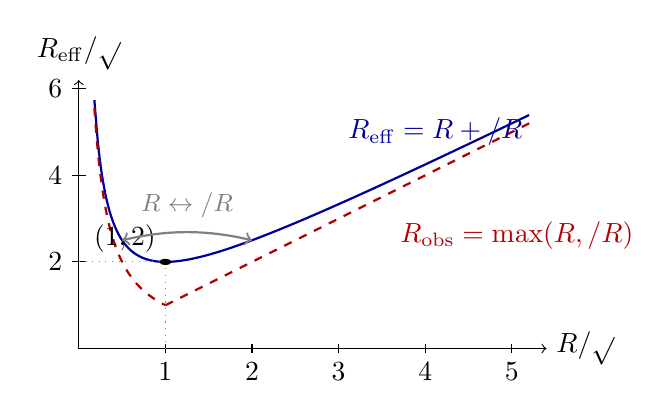
\begin{tikzpicture}[scale=1.0]
 \begin{scope}[xscale=1.1,yscale=0.55]
  \draw[->] (0,0) -- (5.4,0) node[right] {$R/\sqrt{\ap}$};
  \draw[->] (0,0) -- (0,6.2) node[above] {$R_{\rm eff}/\sqrt{\ap}$};
  \foreach \x in {1,2,3,4,5} \draw (\x,0.1)--(\x,-0.1) node[below] {\x};
  \foreach \y in {2,4,6} \draw (0.08,\y)--(-0.08,\y) node[left] {\y};
  % R_eff = r + 1/r
  \draw[thick,blue!60!black,domain=0.18:5.2,samples=120,smooth] plot (\x,{\x+1/\x});
  % R_obs = max(r,1/r)
  \draw[thick,red!70!black,dashed,domain=0.18:1,samples=60] plot (\x,{1/\x});
  \draw[thick,red!70!black,dashed] (1,1)--(5.2,5.2);
  \draw[gray,dotted] (0,2)--(1,2)--(1,0);
  \fill (1,2) circle (2pt) node[above left] {$(1,2)$};
  \node[blue!60!black,anchor=west] at (3.0,5.0) {$R_{\rm eff}=R+\ap/R$};
  \node[red!70!black,anchor=west] at (3.6,2.6) {$R_{\rm obs}=\max(R,\ap/R)$};
  % duality arrows between 1/2 and 2
  \draw[<->,thick,gray] (0.5,2.5) to[bend left=25] (2,2.5);
  \node[gray] at (1.25,3.3) {\small $R\leftrightarrow\ap/R$};
 \end{scope}
\end{tikzpicture}
\caption{The effective scale $R_{\rm eff}$ (solid) and the operational radius $R_{\rm obs}$
(dashed) in string units. Both are invariant under $R\mapsto\ap/R$, which reflects the
horizontal axis about $R=\sqrt{\ap}$ on a logarithmic scale; both are minimal at the
self-dual point, where $R_{\rm eff}=2\sqrt{\ap}$ and $R_{\rm obs}=\sqrt{\ap}$. Every point of
the curve for $R<\sqrt{\ap}$ has a twin for $R>\sqrt{\ap}$.}
\label{fig:dualscale:reff}
\end{figure}

\subsection{A worked example with numbers}

\begin{example}\label{ex:dualscale:numbers}
Take $\ap=1$ (string units) and list, for several radii, the dual radius, the effective scale
and the operational radius:
\begin{center}
\small
\begin{tabular}{@{}cccccc@{}}
\toprule
$R$ & $\tilde R=1/R$ & $x=\ln R$ & $R_{\rm eff}=R+1/R$ & $R_{\rm obs}=\max(R,1/R)$ &
 $R_{\rm eff}/R_{\rm obs}$\\
\midrule
$0.1$ & $10$ & $-2.303$ & $10.1$ & $10$ & $1.01$\\
$0.25$ & $4$ & $-1.386$ & $4.25$ & $4$ & $1.0625$\\
$0.5$ & $2$ & $-0.693$ & $2.5$ & $2$ & $1.25$\\
$1$ & $1$ & $0$ & $2$ & $1$ & $2$\\
$2$ & $0.5$ & $0.693$ & $2.5$ & $2$ & $1.25$\\
$4$ & $0.25$ & $1.386$ & $4.25$ & $4$ & $1.0625$\\
$10$ & $0.1$ & $2.303$ & $10.1$ & $10$ & $1.01$\\
\bottomrule
\end{tabular}
\end{center}
The rows for $R$ and $1/R$ carry the same invariants, as they must. The ratio in the last
column lies between $1$ and $2$ and tends to $1$ away from the self-dual point, which is the
statement $R_{\rm obs}\le R_{\rm eff}\le2R_{\rm obs}$ of \cref{ch:tduality}: the two
candidate ``sizes'' disagree by at most a factor of two, and only near $R=\sqrt{\ap}$. Now
imagine the radius decreasing through the table from top to bottom of the upper half:
$R=0.5\to0.25\to0.1$. The parameter $R$ tends to zero, but $R_{\rm eff}$ has passed through
its minimum at $R=1$ and is \emph{growing}; the string sees a circle that is opening up
again, in Tong's phrase, and the states that become light are the winding states with masses
$|w|R$, i.e. $0.5|w|$, $0.25|w|$, $0.1|w|$.
\end{example}

\begin{pitfallbox}[Common pitfall: $R_{\rm eff}$ is not a length one can lay a ruler along]
It is tempting to read $R_{\rm eff}\ge2\sqrt{\ap}$ as ``the circle is never smaller than
$2\ell_s$''. That is not what the inequality says. The metric radius $R$ is a coordinate on the
moduli space and takes every positive value; nothing stops it from being $10^{-3}\ell_s$. What
the inequality says is that a particular \emph{duality-invariant function} of the modulus is
bounded below. Whether that function is what an experiment measures is a separate question.
\cref{ch:tduality} argued that the lightest Kaluza--Klein tower defines
$R_{\rm obs}=\max(R,\ap/R)\ge\ell_s$; AAL argued that closed-string correlators define a
distance in $(1,\infty)$ \source{AAL §6, ll.~1289--1301}. Both are bounded below for the same
reason as $R_{\rm eff}$, and none of the three is more fundamental than the others without a
further physical argument. Note also that all three concern \emph{closed-string} probes:
Polchinski reports that D-branes appear to probe distances shorter than $\ell_s$, ``in conflict
with the idea that the string length is a minimum distance'' \source{Pol, ll.~3020--3025}, and
open strings have no winding modes at all, so the duality holds for them only together with an
exchange of boundary conditions \source{GPR §1, ll.~380--386}; see \cref{ch:dbranes}.
\end{pitfallbox}

%=====================================================================================
\section{From the circle to the torus: the pair \texorpdfstring{$(G,G^{-1})$}{(G, G inverse)}}
\label{sec:dualscale:torus}

\subsection{The dual scale of a torus metric}

On a torus $T^d$ with constant metric $G_{ij}$ (measured in units of $\ap$, so that a circle of
radius $R$ is $G_{11}=R^2/\ap$) and $B=0$, the zero-mode mass formula of \cref{ch:narain} is
the quadratic form
\begin{equation}\label{eq:dualscale:massform}
 \ap M^2_{\rm zero}=Z^{\mathsf T}\HH(G,0)\,Z,\qquad Z=\begin{pmatrix}w\\ n\end{pmatrix},\qquad
 \HH(G,0)=\begin{pmatrix}G&0\\0&G^{-1}\end{pmatrix},
\end{equation}
in the doubled charge vector $Z=(w,n)$ with the winding block first, which is the convention of
the Lean module described below. The full duality of the torus, the analogue of
\eqref{eq:dualscale:Tmap}, exchanges $w\leftrightarrow n$ and $G\leftrightarrow G^{-1}$; AAL
write it as $(g+b)\mapsto(g+b)^{-1}$ together with the dilaton shift
$\phi\mapsto\phi-\frac12\ln\det(g+b)$ \source{AAL §1, ll.~88--92}. On the generalized metric it
is conjugation by $\eta=\big(\begin{smallmatrix}0&\mathbf1\\\mathbf1&0\end{smallmatrix}\big)$,
\begin{equation}\label{eq:dualscale:eta}
 \eta\,\HH(G,0)\,\eta=\begin{pmatrix}0&\mathbf1\\\mathbf1&0\end{pmatrix}
 \begin{pmatrix}G&0\\0&G^{-1}\end{pmatrix}\begin{pmatrix}0&\mathbf1\\\mathbf1&0\end{pmatrix}
 =\begin{pmatrix}G^{-1}&0\\0&G\end{pmatrix}=\HH(G^{-1},0),
\end{equation}
which is \cref{ch:genmetric}'s ``T-duality is metric inversion''. The pair $(R,\ap/R)$ of the
circle has become the pair of blocks $(G,G^{-1})$ of $\HH$. The circle sum $R+\ap/R$ was the
simplest symmetric function of the pair; the simplest symmetric function of the two blocks is
their combined trace.

\begin{definition}[dual scale of a torus]\label{def:dualscale:D}
For a real invertible $d\times d$ matrix $G$, the \emph{dual scale}\index{dual scale}
\index{generalized metric!trace of} is
\begin{equation}\label{eq:dualscale:D}
 \mathcal D(G)=\Tr\HH(G,0)=\Tr G+\Tr G^{-1}.
\end{equation}
\end{definition}

The second equality is the block structure of \eqref{eq:dualscale:massform}: the trace of a
block-diagonal matrix is the sum of the traces of the blocks, and the off-diagonal blocks
vanish at $B=0$. Three properties are immediate.

\begin{lemma}\label{thm:dualscale:Dprops}
Let $G$ be real and invertible. Then
\begin{enumerate}[label=(\alph*),leftmargin=*]
\item $\mathcal D(G^{-1})=\mathcal D(G)$ (invariance under the full duality $\eta$);
\item $\mathcal D(\mathbf1)=2d$;
\item for $d=1$ and $G=(r^2)$ with $r=R/\sqrt{\ap}\ne0$,
 $\mathcal D(G)=r^2+r^{-2}=\big(r+\tfrac1r\big)^2-2=\dfrac{R_{\rm eff}^2}{\ap}-2$.
\end{enumerate}
\end{lemma}
\begin{proof}
(a) $(G^{-1})^{-1}=G$, so $\mathcal D(G^{-1})=\Tr G^{-1}+\Tr G$. (b) $\Tr\mathbf1=d$ twice.
(c) $(r+1/r)^2=r^2+2+r^{-2}$.
\end{proof}

Part (a) is more than a symmetry of a formula. The trace of a matrix is invariant under
conjugation by an invertible $g$, $\Tr(g\HH g^{-1})=\Tr\HH$, and $\eta^{-1}=\eta$; so
$\mathcal D$ is invariant under $\HH\mapsto\eta\HH\eta$ for any $\HH$, not only at $B=0$.

\begin{pitfallbox}[Common pitfall: $\mathcal D$ is not invariant under all of $\Odd{d}$]
The duality group of \cref{ch:odd} acts on the generalized metric by
$\HH\mapsto g^{\mathsf T}\HH g$, and $\Tr(g^{\mathsf T}\HH g)=\Tr(\HH gg^{\mathsf T})$ equals
$\Tr\HH$ only when $gg^{\mathsf T}=\mathbf1$. The inversion $\eta$ is orthogonal, so
$\mathcal D$ survives it; a change of lattice basis $G\mapsto A^{\mathsf T}GA$ with
$A\in GL(d,\Z)$ is orthogonal only when $A$ is a signed permutation, and a $B$-shift is never
orthogonal. Concretely, the hexagonal torus
$G=\big(\begin{smallmatrix}1&1/2\\1/2&1\end{smallmatrix}\big)$ has $\mathcal D=14/3$, but in
the basis $A=\big(\begin{smallmatrix}1&1\\0&1\end{smallmatrix}\big)$ the same torus is
$A^{\mathsf T}GA=\big(\begin{smallmatrix}1&3/2\\3/2&3\end{smallmatrix}\big)$ with
$\mathcal D=28/3$ (symbolic check). For $d=1$ the only basis changes are $\pm1$ and the
problem disappears, which is why the circle statement is clean. For $d\ge2$, $\mathcal D$ is a
function on the space of metrics \emph{in a chosen basis}; the bound of
\cref{thm:dualscale:main} holds in every basis, but the number $\mathcal D(G)$ itself is not an
invariant of the torus. A basis-independent version would take the minimum of $\mathcal D$ over
the $GL(d,\Z)$-orbit (a reduction-theory statement not formalized here, and not made in the
sources); this is one of the gaps between the theorem and the proposal.
\end{pitfallbox}

\subsection{The bound \texorpdfstring{$\Tr G+\Tr G^{-1}\ge2d$}{tr G + tr G inverse >= 2d}}

\begin{theorem}[dual-scale bound]\label{thm:dualscale:main}
Let $G$ be a real symmetric positive definite $d\times d$ matrix. Then
\begin{equation}\label{eq:dualscale:bound}
 \Tr G+\Tr G^{-1}\;\ge\;2d,
\end{equation}
with equality if and only if $G=\mathbf1$.
\end{theorem}

\begin{proof}[First proof, by the spectral theorem]
A real symmetric matrix is orthogonally diagonalizable: $G=O^{\mathsf T}\Lambda O$ with
$O^{\mathsf T}O=\mathbf1$ and $\Lambda=\diag(\lambda_1,\dots,\lambda_d)$, and positive
definiteness means every $\lambda_i>0$. Then $G^{-1}=O^{\mathsf T}\Lambda^{-1}O$, and since the
trace is invariant under conjugation,
\[
 \Tr G+\Tr G^{-1}=\sum_{i=1}^d\Big(\lambda_i+\frac1{\lambda_i}\Big).
\]
Each term is the circle bound of \cref{thm:dualscale:circle} with $\ap=1$:
$\lambda+1/\lambda-2=(\lambda-1)^2/\lambda\ge0$, with equality only at $\lambda=1$. Summing,
$\Tr G+\Tr G^{-1}-2d=\sum_i(\lambda_i-1)^2/\lambda_i\ge0$, and equality forces every
$\lambda_i=1$, i.e. $\Lambda=\mathbf1$ and $G=O^{\mathsf T}O=\mathbf1$.
\end{proof}

The spectral proof is the natural one for a physicist: the torus metric can always be brought
to diagonal form $\diag(r_1^2,\dots,r_d^2)$ by an orthogonal (not integral!) change of
coordinates, and then $\mathcal D=\sum_i(r_i^2+r_i^{-2})$ is a sum of circle invariants. But it
uses a theorem of some depth, and a proof assistant will ask for it to be supplied. The proof
that was actually formalized uses less.

\begin{proof}[Second proof, by a positive sandwich]
Step 1 (an identity). Using $GG^{-1}=G^{-1}G=\mathbf1$,
\begin{equation}\label{eq:dualscale:sandwich}
 (G-\mathbf1)\,G^{-1}\,(G-\mathbf1)
 =(G-\mathbf1)(\mathbf1-G^{-1})
 =G-\mathbf1-\mathbf1+G^{-1}
 =(G-\mathbf1)-(\mathbf1-G^{-1}).
\end{equation}
Taking the trace, $\Tr\big[(G-\mathbf1)G^{-1}(G-\mathbf1)\big]=\Tr G+\Tr G^{-1}-2d$. (Symbolic
check on a general symmetric $2\times2$ matrix: the identity and its trace both hold.)

Step 2 (a sign). The inverse of a positive definite matrix is positive definite, hence positive
semidefinite: $v^{\mathsf T}G^{-1}v=(G^{-1}v)^{\mathsf T}G(G^{-1}v)\ge0$. For any matrix $M$
and positive semidefinite $P$, the sandwich $M^{\mathsf T}PM$ is positive semidefinite, since
$v^{\mathsf T}M^{\mathsf T}PMv=(Mv)^{\mathsf T}P(Mv)\ge0$. Apply this with $M=G-\mathbf1$,
which is symmetric, and $P=G^{-1}$.

Step 3 (trace of a positive semidefinite matrix). If $S$ is positive semidefinite then
$S_{ii}=e_i^{\mathsf T}Se_i\ge0$ for each basis vector $e_i$, so $\Tr S=\sum_iS_{ii}\ge0$.
Combining the three steps, $\Tr G+\Tr G^{-1}-2d\ge0$.

Uniqueness. Suppose equality holds. Then the positive semidefinite matrix
$S=(G-\mathbf1)G^{-1}(G-\mathbf1)$ has zero trace, so each $S_{ii}=0$; a positive
semidefinite matrix with vanishing diagonal is zero (its $2\times2$ principal minors
$S_{ii}S_{jj}-S_{ij}^2\ge0$ force $S_{ij}=0$). Then for every $v$,
$0=v^{\mathsf T}Sv=u^{\mathsf T}G^{-1}u$ with $u=(G-\mathbf1)v$, and positive definiteness of
$G^{-1}$ gives $u=0$; so $G-\mathbf1$ annihilates every vector, and $G=\mathbf1$.
\end{proof}

No eigenvalue is computed in the second proof. Its ingredients are: the algebra of
\eqref{eq:dualscale:sandwich}, the facts that the inverse of a positive definite matrix is
positive semidefinite and that sandwiches preserve positive semidefiniteness, and the
nonnegativity of the trace of a positive semidefinite matrix. Each of these is a lemma in
Mathlib, and \cref{sec:dualscale:lean} shows the proof assembled from them. When this chapter
was first written the uniqueness paragraph was not formalized: Lean proved the inequality and,
separately, that the value $2d$ is attained at $G=\mathbf1$. It now also proves the converse,
\lean{dualScale\_eq\_iff}: for positive definite $G$, $\Tr G+\Tr G^{-1}=2d$ if and only if
$G=\mathbf1$. The Lean proof follows the paragraph above with one difference: where we used
$2\times2$ minors to pass from zero trace to $S=0$, Lean calls Mathlib's
\lean{Matrix.PosSemidef.trace\_eq\_zero\_iff}, which goes through the spectral theorem. So the
inequality is still proved without eigenvalues, but the equality case, in Lean, is not.

\begin{corollary}\label{thm:dualscale:corollaries}
For positive definite $G$ and antisymmetric $B$:
\begin{enumerate}[label=(\alph*),leftmargin=*]
\item $\Tr\HH(G,B)=\Tr G+\Tr G^{-1}+\Tr(B^{\mathsf T}G^{-1}B)\ge\Tr\HH(G,0)\ge2d$;
\item in the variables $\lambda_i=\ee^{2x_i}$, $\mathcal D(G)=2\sum_i\cosh2x_i$, an even
 function of each $x_i$;
\item for the circle, $\mathcal D\ge2$ is equivalent to $R_{\rm eff}\ge2\sqrt{\ap}$.
\end{enumerate}
\end{corollary}
\begin{proof}
(a) From the block form of \cref{ch:genmetric}, $\Tr\HH(G,B)=\Tr(G-BG^{-1}B)+\Tr G^{-1}$, and
$-BG^{-1}B=B^{\mathsf T}G^{-1}B$ is a sandwich of the positive semidefinite $G^{-1}$, hence has
nonnegative trace. (Symbolic check: for $d=2$ the excess is $\beta^2\Tr G/\det G$ where
$B_{12}=\beta$.) So a $B$-field can only increase the dual scale, and the bound at $B=0$ is the
sharp one. (b) Substitute $\lambda_i+\lambda_i^{-1}=2\cosh2x_i$ into the spectral proof.
(c) \cref{thm:dualscale:Dprops}(c): $\mathcal D=R_{\rm eff}^2/\ap-2\ge2$ if and only if
$R_{\rm eff}^2\ge4\ap$.
\end{proof}

\begin{figure}[t]
\centering
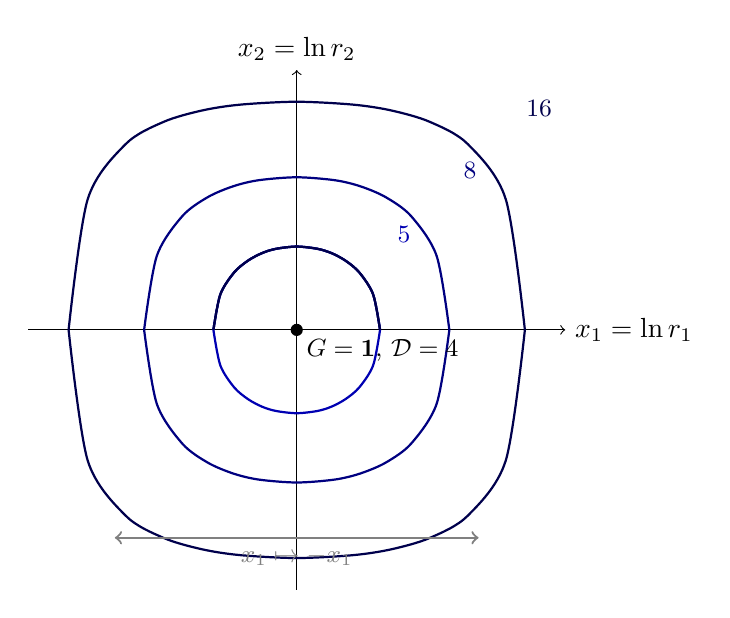
\begin{tikzpicture}[scale=2.2]
 \draw[->] (-1.55,0) -- (1.55,0) node[right] {$x_1=\ln r_1$};
 \draw[->] (0,-1.5) -- (0,1.5) node[above] {$x_2=\ln r_2$};
 \foreach \c/\col in {2.5/blue!70!black,4/blue!50!black,8/blue!30!black}{
  \draw[thick,\col] plot[smooth] coordinates {
   (-0.481,0.0) (-0.441,0.205) (-0.361,0.332) (-0.281,0.4) (-0.201,0.443) (-0.12,0.468)
   (0.0,0.481) (0.12,0.468) (0.201,0.443) (0.281,0.4) (0.361,0.332) (0.441,0.205) (0.481,0.0)};
 }
 \draw[thick,blue!70!black] plot[smooth] coordinates {
   (-0.481,0.0) (-0.441,-0.205) (-0.361,-0.332) (-0.281,-0.4) (-0.201,-0.443) (-0.12,-0.468)
   (0.0,-0.481) (0.12,-0.468) (0.201,-0.443) (0.281,-0.4) (0.361,-0.332) (0.441,-0.205) (0.481,0.0)};
 \draw[thick,blue!50!black] plot[smooth] coordinates {
   (-0.881,0.0) (-0.808,0.426) (-0.661,0.656) (-0.514,0.766) (-0.367,0.829) (-0.22,0.864)
   (0.0,0.881) (0.22,0.864) (0.367,0.829) (0.514,0.766) (0.661,0.656) (0.808,0.426) (0.881,0.0)};
 \draw[thick,blue!50!black] plot[smooth] coordinates {
   (-0.881,0.0) (-0.808,-0.426) (-0.661,-0.656) (-0.514,-0.766) (-0.367,-0.829) (-0.22,-0.864)
   (0.0,-0.881) (0.22,-0.864) (0.367,-0.829) (0.514,-0.766) (0.661,-0.656) (0.808,-0.426) (0.881,0.0)};
 \draw[thick,blue!30!black] plot[smooth] coordinates {
   (-1.317,0.0) (-1.207,0.753) (-0.988,1.072) (-0.768,1.201) (-0.549,1.266) (-0.329,1.3)
   (0.0,1.317) (0.329,1.3) (0.549,1.266) (0.768,1.201) (0.988,1.072) (1.207,0.753) (1.317,0.0)};
 \draw[thick,blue!30!black] plot[smooth] coordinates {
   (-1.317,0.0) (-1.207,-0.753) (-0.988,-1.072) (-0.768,-1.201) (-0.549,-1.266) (-0.329,-1.3)
   (0.0,-1.317) (0.329,-1.3) (0.549,-1.266) (0.768,-1.201) (0.988,-1.072) (1.207,-0.753) (1.317,0.0)};
 \fill (0,0) circle (1pt);
 \node[below right] at (0,0) {\small $G=\mathbf1$, $\mathcal D=4$};
 \node[blue!70!black] at (0.62,0.55) {\small $5$};
 \node[blue!50!black] at (1.0,0.92) {\small $8$};
 \node[blue!30!black] at (1.4,1.28) {\small $16$};
 \draw[<->,gray,thick] (-1.05,-1.2) -- (1.05,-1.2) node[midway,below] {\small $x_1\mapsto-x_1$};
\end{tikzpicture}
\caption{Level sets of the dual scale $\mathcal D=2(\cosh2x_1+\cosh2x_2)$ for diagonal
metrics $G=\diag(\ee^{2x_1},\ee^{2x_2})$ on $T^2$, at the values $5$, $8$ and $16$. The
function is even in each coordinate, the four reflections $x_i\mapsto-x_i$ being the
factorized dualities of \cref{ch:odd}, and it has a single minimum $2d=4$ at the origin.}
\label{fig:dualscale:levels}
\end{figure}

\subsection{Worked examples}

\begin{example}[a rectangular torus]\label{ex:dualscale:rect}
Take $d=2$ and $G=\diag(4,\tfrac14)$, i.e. $R_1=2\ell_s$ and $R_2=\ell_s/2$. Then
$G^{-1}=\diag(\tfrac14,4)$ and $\mathcal D=4+\tfrac14+\tfrac14+4=8.5\ge4$. The full duality
$G\mapsto G^{-1}$ exchanges the two radii, $(2,\tfrac12)\mapsto(\tfrac12,2)$, and leaves
$\mathcal D$ unchanged, as \cref{thm:dualscale:Dprops}(a) requires. The factorized duality in
the first direction alone, $R_1\mapsto\ap/R_1$, sends $G$ to $\diag(\tfrac14,\tfrac14)$, with
$\mathcal D=\tfrac12+8=8.5$ again; the torus with both radii equal to $\ell_s/2$ has the same
dual scale as the one with radii $(2,\tfrac12)$, because $\mathcal D$ is a sum of circle
invariants and each is even in $x_i$. Contrast $\det G$, which is $1$ for the first torus and
$1/16$ for the second: the determinant is invariant under $SL(2,\Z)$ basis changes, which
$\mathcal D$ is not, but changes under factorized dualities, which $\mathcal D$ survives.
\end{example}

\begin{example}[a sheared torus with unit determinant]\label{ex:dualscale:shear}
Take $G=\big(\begin{smallmatrix}5&2\\2&1\end{smallmatrix}\big)$, which is positive definite
($\det G=1$, $G_{11}>0$) and not diagonal. Its inverse is
$G^{-1}=\big(\begin{smallmatrix}1&-2\\-2&5\end{smallmatrix}\big)$, so
$\mathcal D=6+6=12$. The eigenvalues are $\lambda_\pm=3\pm2\sqrt2$, with
$\lambda_+\lambda_-=1$ and $\lambda_++\lambda_-=6$; the spectral formula gives
$\sum(\lambda+1/\lambda)=2(\lambda_++\lambda_-)=12$, in agreement. In the sandwich proof,
$G-\mathbf1=\big(\begin{smallmatrix}4&2\\2&0\end{smallmatrix}\big)$ and
\[
 (G-\mathbf1)G^{-1}(G-\mathbf1)
 =\begin{pmatrix}4&2\\2&0\end{pmatrix}\begin{pmatrix}1&-2\\-2&5\end{pmatrix}
  \begin{pmatrix}4&2\\2&0\end{pmatrix}
 =\begin{pmatrix}0&2\\2&-4\end{pmatrix}\begin{pmatrix}4&2\\2&0\end{pmatrix}
 =\begin{pmatrix}4&0\\0&4\end{pmatrix},
\]
whose trace is $8=12-2\cdot2$, as \eqref{eq:dualscale:sandwich} predicts. Note that
$\big(\begin{smallmatrix}0&2\\2&-4\end{smallmatrix}\big)$ is not positive semidefinite---only the
completed sandwich is.
\end{example}

\begin{example}[the hexagonal torus]\label{ex:dualscale:hex}
$G=\big(\begin{smallmatrix}1&1/2\\1/2&1\end{smallmatrix}\big)$ has eigenvalues $\tfrac32$ and
$\tfrac12$ (eigenvectors $(1,1)$ and $(1,-1)$) and
$G^{-1}=\tfrac43\big(\begin{smallmatrix}1&-1/2\\-1/2&1\end{smallmatrix}\big)$, so
$\mathcal D=2+\tfrac83=\tfrac{14}3\approx4.67$; the spectral formula gives
$\tfrac32+\tfrac23+\tfrac12+2=\tfrac{14}3$. This is the smallest value among the three
examples, as befits the torus closest to $G=\mathbf1$, but it is still strictly above $4$.
\end{example}

%=====================================================================================
\section{What the older libraries model: arithmetic shadows}\label{sec:dualscale:shadows}

Four older Lean modules of this project are named in the atlas as formalizing the dual-scale
principle. They were written before the matrix statement of \cref{sec:dualscale:torus} and
they model radii by natural numbers, integers or positive rationals. Following the rule of
this book, we describe them as \emph{arithmetic shadows}\index{arithmetic shadow}: each proves
an exact arithmetic fact, and each docstring attaches to that fact a physical reading which the
statement does not carry. Reading the statements literally is the skill this section trains.

\subsection{Positive rational scales and the piecewise radius}

\index{Lean!buscherDual@\texttt{buscherDual}}\index{Lean!genesis\_no\_singularity@\texttt{genesis\_no\_singularity}}
\begin{leanbox}[In Lean: \texttt{DualScaleM24Formalization/DualScale/EffectiveMetric.lean}]
\begin{leancode}
structure PosScale where
  num : Nat
  den : Nat
  h_num : 0 < num
  h_den : 0 < den

def scaleEq (s1 s2 : PosScale) : Prop := s1.num * s2.den = s2.num * s1.den
def scaleLt (s1 s2 : PosScale) : Prop := s1.num * s2.den < s2.num * s1.den

def buscherDual (alpha : PosScale) (R : PosScale) : PosScale :=
  ⟨alpha.num * R.den, alpha.den * R.num,
   Nat.mul_pos alpha.h_num R.h_den, Nat.mul_pos alpha.h_den R.h_num⟩

theorem buscher_involution (alpha : PosScale) (R : PosScale) :
    scaleEq (buscherDual alpha (buscherDual alpha R)) R := by ...

def effectiveRadius (cutoff : PosScale) (alpha : PosScale) (R : PosScale) :
    PosScale :=
  if scaleLt R cutoff then buscherDual alpha R else R

theorem genesis_no_singularity (cutoff : PosScale) (alpha : PosScale)
    (R : PosScale) :
    0 < (effectiveRadius cutoff alpha R).num ∧
    0 < (effectiveRadius cutoff alpha R).den := by ...

theorem self_dual_symmetric (alpha : PosScale) :
    scaleEq (buscherDual alpha alpha) ⟨1, 1, by decide, by decide⟩ := by ...
\end{leancode}
\textbf{Reading.} A \lean{PosScale} is a positive rational written as a fraction of positive
naturals; two are \lean{scaleEq} when they cross-multiply to the same value. \lean{buscherDual
alpha R} is the fraction $\ap/R$, and \lean{buscher\_involution} says $\ap/(\ap/R)=R$ as
rationals---the map $R\mapsto\ap/R$ is an involution, \TA{} for positive rationals. The
function \lean{effectiveRadius} is the piecewise \emph{operational} radius of
\cref{ch:tduality}, $\ap/R$ below a cutoff and $R$ above it, with the cutoff a free parameter
rather than $\sqrt{\ap}$ (which is not rational). \lean{genesis\_no\_singularity} states
that the numerator and denominator of this fraction are positive. Literally: \emph{a
positive rational is positive}, in both branches of the definition. It does not state the
bound $R_{\rm eff}\ge2\sqrt{\ap}$, nor that any function is bounded away from zero
uniformly---for a cutoff $c$, the value $\ap/R$ with $R$ just below $c$ can be as small as
$\ap/c$, and $R$ itself just above $c$ is $c$; and it says nothing about spacetime, curvature or
a bounce. \lean{self\_dual\_symmetric} says $\ap/\ap=1$.

\textbf{What a faithful version needs.} Real (or at least ordered-field) radii; the function
$R+\ap/R$ or $\max(R,\ap/R)$; the inequality of \cref{thm:dualscale:circle}. All of this is
exactly what \lean{circle\_effective\_scale\_ge\_two} in \cref{sec:dualscale:lean} provides
over $\R$, which is why the newer module was written.
\end{leanbox}

\subsection{Dual pairs of integers}

\index{Lean!isDualPair@\texttt{isDualPair}}
\begin{leanbox}[In Lean: \texttt{StringTheoryFoundation/Duality/DualScale.lean}]
\begin{leancode}
def dualLength (L_star L : Float) : Float := (L_star * L_star) / L

def isDualPair (L_star L L_dual : Int) : Prop := L * L_dual = L_star * L_star

theorem dual_pair_symmetric (L_star L L_dual : Int)
    (h : isDualPair L_star L L_dual) : isDualPair L_star L_dual L := by ...

theorem self_dual_at_crossover (L_star : Int) :
    isDualPair L_star L_star L_star := by rfl

theorem dual_product_invariant (L_star L L_dual : Int)
    (h : isDualPair L_star L L_dual) : L * L_dual = L_star * L_star := h
\end{leancode}
\textbf{Reading.} Two integers form a dual pair for the crossover scale $L_*$ when their
product is $L_*^2$; this is the relation $R\tilde R=\ap$ with $L_*=\ell_s$.
\lean{dual\_pair\_symmetric} is the commutativity of integer multiplication;
\lean{self\_dual\_at\_crossover} is $L_*\cdot L_*=L_*\cdot L_*$, proved by \lean{rfl};
\lean{dual\_product\_invariant} returns its hypothesis unchanged. \lean{dualLength} is a
\lean{Float} function about which nothing is proved (floating-point arithmetic has no useful
algebraic theorems). These are \TA{} as statements about integers, and they are the weakest
possible shadow of the principle: the invariance of the product, which is a tautology, and
none of the inequality.
\end{leanbox}

\subsection{The numerator of \texorpdfstring{$R\cdot R_{\rm eff}$}{R times R\_eff} over the naturals}

\index{Lean!self\_dual\_is\_global\_minimum@\texttt{self\_dual\_is\_global\_minimum}}
\begin{leanbox}[In Lean: \texttt{DualScaleValidation/UseCase1\_ModuliStabilization.lean}]
\begin{leancode}
def alpha_prime : Nat := 1

def effective_dual_scale_numerator (R : Nat) : Nat := R * R + alpha_prime

theorem buscher_log_involution (x : Int) : -(-x) = x := by omega

theorem dual_scale_self_dual_value : effective_dual_scale_numerator 1 = 2 := by rfl

theorem self_dual_is_global_minimum (R : Nat) (h : R ≥ 1) :
    effective_dual_scale_numerator R ≥ 2 := by ...

def moduli_potential (phi phi_0 : Int) : Int := (phi - phi_0) * (phi - phi_0)

theorem moduli_potential_nonneg (phi phi_0 : Int) :
    moduli_potential phi phi_0 ≥ 0 := by ...

theorem moduli_potential_zero_iff (phi phi_0 : Int) :
    moduli_potential phi phi_0 = 0 ↔ phi = phi_0 := by ...
\end{leancode}
\textbf{Reading.} With $\ap=1$, the natural number $R^2+1$ is $R\cdot R_{\rm eff}(R)$, the
numerator of the effective scale. \lean{buscher\_log\_involution} is $-(-x)=x$ on $\Z$, the
statement that the reflection $x\mapsto-x$ of the logarithmic radius is an involution.
\lean{dual\_scale\_self\_dual\_value} is $1+1=2$. \lean{self\_dual\_is\_global\_minimum}
says: for a natural number $R\ge1$, $R^2+1\ge2$. This must be read with care, because its name
promises more than it delivers. The bound $R_{\rm eff}\ge2$ is $R^2+1\ge2R$, i.e.
$(R-1)^2\ge0$; the theorem proves only $R^2+1\ge2$, which for $R\ge1$ is the weaker
statement $R\cdot R_{\rm eff}\ge2$, hence $R_{\rm eff}\ge2/R$, and $2/R\le2$. At $R=3$ the
theorem gives $10\ge2$ while the dual-scale bound requires $10\ge6$. Moreover the hypothesis
$R\ge1$ over $\N$ excludes the sub-string radii $0<R<1$ where the ``bounce'' of the docstring
would take place: there are no such natural numbers. So the theorem is \TA{} as arithmetic,
but it is not the statement that the self-dual point is a global minimum; that statement, over
$\R$ and with the correct inequality, is \lean{circle\_effective\_scale\_ge\_two}. The
\lean{moduli\_potential} theorems say that the integer $(\phi-\phi_0)^2$ is nonnegative and
vanishes exactly at $\phi=\phi_0$---a correct toy of a potential with a unique minimum, with no
connection to the dual scale beyond the analogy that both have a unique minimum, and none to
the flux potentials of \cref{ch:stabilization}. The module also records
\lean{dft\_doubled\_dimension\_10d}: $2\cdot10=20$.
\end{leanbox}

\subsection{The symmetric-square lock}

The module \texttt{DualScaleM24Formalization/DualScale/Sym2Lock.lean} is grouped with the
dual-scale files because its docstring presents it as the ``micro--macro bridge'' of the
programme: a linear second-order recurrence on a ``microscopic'' fibre is squared to produce a
third-order recurrence on ``macroscopic'' observables. The mathematics is an exercise about
linear recurrences, and it is worth doing by hand before reading the Lean.

\begin{lemma}\label{thm:dualscale:sym2}
Let $u_{n+2}=a\,u_{n+1}+b\,u_n$ with characteristic roots $\lambda_1,\lambda_2$
($\lambda^2-a\lambda-b=0$, so $\lambda_1+\lambda_2=a$, $\lambda_1\lambda_2=-b$). Then
$v_n=u_n^2$ satisfies $v_{n+3}=c_2v_{n+2}+c_1v_{n+1}+c_0v_n$ with
\begin{equation}\label{eq:dualscale:sym2}
 c_2=a^2+b,\qquad c_1=b\,(a^2+b),\qquad c_0=-b^3 .
\end{equation}
\end{lemma}
\begin{proof}
For distinct roots, $u_n=\alpha\lambda_1^n+\beta\lambda_2^n$, so
$v_n=\alpha^2\lambda_1^{2n}+2\alpha\beta(\lambda_1\lambda_2)^n+\beta^2\lambda_2^{2n}$ is a
linear combination of the three geometric sequences with ratios
$\lambda_1^2,\lambda_1\lambda_2,\lambda_2^2$---the weights of the symmetric square
$\mathrm{Sym}^2$ of the two-dimensional representation. Hence $v$ satisfies the recurrence
whose characteristic polynomial is
$(x-\lambda_1^2)(x-\lambda_2^2)(x-\lambda_1\lambda_2)=x^3-c_2x^2-c_1x-c_0$ with
$c_2=\lambda_1^2+\lambda_2^2+\lambda_1\lambda_2=(a^2+2b)-b=a^2+b$,
$c_1=-\big[\lambda_1^2\lambda_2^2+\lambda_1\lambda_2(\lambda_1^2+\lambda_2^2)\big]
 =-\big[b^2-b(a^2+2b)\big]=b(a^2+b)$ and $c_0=(\lambda_1\lambda_2)^3=-b^3$. The case of a
repeated root follows by continuity in $(a,b)$. (Symbolic check: all three coefficients agree
after substituting the roots.)
\end{proof}

\index{Lean!sym2Lock@\texttt{sym2Lock}}
\begin{leanbox}[In Lean: \texttt{DualScaleM24Formalization/DualScale/Sym2Lock.lean}]
\begin{leancode}
structure MicroL2Operator where
  a : Int
  b : Int

structure MacroL3Operator where
  c2 : Int
  c1 : Int
  c0 : Int

def stepL3 (op : MacroL3Operator) (v2 v1 v0 : Int) : Int :=
  op.c2 * v2 + op.c1 * v1 + op.c0 * v0

def sym2Lock (op : MicroL2Operator) : MacroL3Operator := {
  c2 := op.a * op.a + op.b
  c1 := op.b * (op.a * op.a + op.b)
  c0 := - (op.b * op.b * op.b) }

theorem sym2_fibonacci_verification :
    let l2 : MicroL2Operator := ⟨1, 1⟩
    let l3 := sym2Lock l2
    l3.c2 = 2 ∧ l3.c1 = 2 ∧ l3.c0 = -1 ∧
    stepL3 l3 4 1 1 = 9 ∧ stepL3 l3 9 4 1 = 25 ∧ stepL3 l3 25 9 4 = 64 := by
  decide

def sym2Det (l2 : MicroL2Operator) : Int := - (sym2Lock l2).c0

theorem sym2_det_identity (l2 : MicroL2Operator) :
    sym2Det l2 = l2.b * l2.b * l2.b := by ...
\end{leancode}
\textbf{Reading.} \lean{sym2Lock} is the map $(a,b)\mapsto(c_2,c_1,c_0)$ of
\eqref{eq:dualscale:sym2} on integers. The Lean library does \emph{not} prove
\cref{thm:dualscale:sym2}: it proves, by \lean{decide}, that for the Fibonacci data
$(a,b)=(1,1)$ the coefficients are $(2,2,-1)$ and that the squares $1,1,4,9,25,64$ satisfy
three instances of the recurrence ($9=2\cdot4+2\cdot1-1$, and so on), with similar checks for
the Pell data $(2,1)$ and for $(3,-1)$ (\lean{sym2\_pell\_verification},
\lean{sym2\_modular\_attractor\_verification}). \lean{sym2\_det\_identity} says $-c_0=b^3$,
which is the definition of $c_0$. These are \TA{} as finite integer computations. The general
lemma is proved above by hand and is standard; its physical reading as a bridge between
``microscopic'' and ``macroscopic'' dynamics, and the applications listed in the docstring, are
\TC{} and are not examined further in this book.
\end{leanbox}

\subsection{The observables module}

\texttt{DualScaleValidation/Observables.lean} imports the module of the previous subsection and
certifies four arithmetic facts about numbers that appear in the programme's phenomenological
proposals:
\begin{itemize}[leftmargin=*,nosep]
\item $110/27720$ reduces to $1/252$ (\lean{tensor\_to\_scalar\_ratio\_reduction});
\item $1/252$ lies in $[0.003,0.005]$, $965/1000$ lies in $[0.950,0.980]$ and $283$ lies in
 $[270,295]$ (three window theorems);
\item two integer constants equal $-1$ and $0$ (\lean{dark\_energy\_cosmological\_constant});
\item the conjunction of the above (\lean{observables\_windows\_master\_contract}).
\end{itemize}
The module's own docstring is explicit that these are ``Tier A for its arithmetic only'' and that the relations
between the integers and observed quantities are ``post-hoc numerical matches'' with ``no
dynamical or field-theoretic derivation'', in one case in tension with current data. We follow
the docstring: the arithmetic is \TA, the identification of any of these numbers with a
cosmological observable is \TC, and the module contains no theorem connecting them to
$R_{\rm eff}$ or to $\Tr G+\Tr G^{-1}$. A reader looking for ``predictions of the dual-scale
principle'' will not find them in the kernel-checked corpus.

%=====================================================================================
\section{Separating the tiers}\label{sec:dualscale:tiers}

The principle of \cref{sec:dualscale:thesis} was stated in three tiers, and the intervening
sections have supplied the evidence for each. We now put the pieces side by side, because the
most common error in reading this programme's documents---and, to be candid, in some of the
docstrings quoted above---is to let the certainty of tier~A leak into tiers~L and~C.

\subsection{What the inequality does not say}

\cref{thm:dualscale:main} is a statement about a function on the space of positive definite
matrices. To turn it into a statement about physics one needs at least the following, none of
which is a theorem in this book's library.

\begin{enumerate}[leftmargin=*]
\item \emph{An identification of the variable.} The matrix $G$ must be the metric of a flat
 torus in a string background, in units of $\ap$, in a fixed lattice basis. In Lean, $G$ is any
 real matrix; the identification is made in a docstring. This step can never be Tier~A.
\item \emph{A choice of observable.} One must argue that $\Tr G+\Tr G^{-1}$, rather than
 $\max$-type invariants, the minimum over the $GL(d,\Z)$-orbit, or a function of the full
 $\HH(G,B)$, is what some measurement returns. For the circle the literature offers
 arguments for a minimal \emph{measured} radius (\TL), but for $R_{\rm obs}$ or for the
 correlator-defined distance of AAL, not specifically for $R_{\rm eff}$; \cref{ch:tduality}
 showed that the candidates agree within a factor of two, which is a reason to be relaxed about
 the choice, not a derivation of it.
\item \emph{Dynamics.} A bound on a function of the moduli says nothing about how the moduli
 evolve. That a contracting universe is driven to the self-dual radius is a dynamical statement
 which string gas cosmology derives from the pressures of winding and momentum modes under
 stated assumptions (equal populations, the dilaton running to weak coupling, adiabatic
 evolution) \source{BW §IV, ll.~1110--1134}; \cref{ch:cosmology} presents it. The inequality
 by itself does not prevent the metric radius $R$ from reaching zero; it only says that
 $R_{\rm eff}$ would then be large.
\item \emph{Beyond free strings.} The mass formula \eqref{eq:dualscale:M2} is the free
 spectrum. GPR are careful to say that the equivalence of small and large radius as a statement
 about the \emph{interacting} string requires the higher-genus contributions, which they prove
 in their next section \source{GPR §2.2, ll.~784--793}; the extension to curved backgrounds,
 to D-brane probes and to non-perturbative physics is each a separate question
 (\cref{ch:buscher,ch:dbranes,ch:swampland}).
\end{enumerate}

\subsection{The tiers, side by side}

\begin{center}
\small
\begin{tabular}{@{}p{0.54\textwidth}p{0.34\textwidth}c@{}}
\toprule
Statement & Evidence & Tier\\
\midrule
$R+\ap/R\ge2\sqrt{\ap}$ for real $R>0$ (units $\ap=1$) &
 \lean{circle\_effective\_scale\_ge\_two} & \TA\\
$\Tr G+\Tr G^{-1}\ge2d$ for positive definite real $G$, all $d$ &
 \lean{dualScale\_ge} & \TA\\
$\mathcal D(G^{-1})=\mathcal D(G)$ for invertible real $G$ & \lean{dualScale\_inv} & \TA\\
$\mathcal D(\mathbf1)=2d$ (the bound is attained) & \lean{dualScale\_one} & \TA\\
$\mathcal D(R^2)=(R+1/R)^2-2$ for the circle & \lean{dualScale\_circle} & \TA\\
$\ap/(\ap/R)=R$ for positive rationals; $-(-x)=x$ on $\Z$ &
 \lean{buscher\_involution}, \lean{buscher\_log\_involution} & \TA\\
Equality in \eqref{eq:dualscale:bound} only at $G=\mathbf1$ & hand proof,
 \cref{thm:dualscale:main} & ---\\
$\Tr\HH(G,B)\ge\Tr\HH(G,0)$ & hand proof, \cref{thm:dualscale:corollaries} & ---\\
\midrule
Closed strings cannot distinguish $R$ from $\ap/R$; a minimal length in this sense &
 GPR §2.2, Tong §8.3, AAL §6 & \TL\\
One-loop partition function on a circle $\propto R+1/R$ & GPR §1 & \TL\\
Balanced string gas: $\rho\propto R+1/R$, pressure vanishes at $R=\sqrt{\ap}$ &
 BW §III--IV & \TL\\
Winding modes annihilate in at most three large dimensions (Brandenberger--Vafa) &
 BW §IV & \TL\\
\midrule
$R_{\rm eff}$ (resp.\ $\Tr G+\Tr G^{-1}$) is \emph{the} physical size & this programme & \TC\\
The bound regulates the cosmological singularity; a bounce & this programme; docstrings of
 \cref{sec:dualscale:shadows} & \TC\\
$\mathrm{Sym}^2$ lock as a micro--macro bridge; observables of \texttt{Observables.lean} &
 this programme & \TC\\
\bottomrule
\end{tabular}
\end{center}

\begin{historybox}[The Brandenberger--Vafa argument]
The idea that winding strings control the size of compact dimensions predates T-duality's use
as a minimal-length argument in cosmology. As Battefeld and Watson recount it, Brandenberger
and Vafa (1989) argued that winding strings ``can maintain equilibrium in at most three spatial
dimensions'', because $p$-dimensional objects generically intersect in at most $2p+1$
dimensions and string interactions occur at intersections; once winding modes annihilate with
anti-winding modes, three dimensions ``would be free to expand while the remaining six should
remain confined by winding modes near the string scale'' \source{BW §IV, ll.~921--928}. The
later observation that a balanced gas is driven to the self-dual radius (Watson and
Brandenberger 2003, as cited by BW) is what connects this picture to $R_{\rm eff}$. Battefeld
and Watson also stress that a gas of purely winding modes is \emph{not} enough to stabilize
the extra dimensions \source{BW abstract, ll.~165--166}, which is a first warning that the
picture depends on details.
\end{historybox}

%=====================================================================================
\section{What the machine has checked}\label{sec:dualscale:lean}

The module \texttt{TraceBound.lean} in \texttt{DualScaleStream2/DualScale/} formalizes
\cref{def:dualscale:D}, \cref{thm:dualscale:Dprops} and the inequality of
\cref{thm:dualscale:main} over $\R$, for every $d$, on top of the generalized metric
\lean{genMetric} of \cref{ch:genmetric}. It is a short file, and we go through all of it.

\index{Lean!dualScale@\texttt{dualScale}}\index{Lean!dualScale\_eq@\texttt{dualScale\_eq}}
\index{Lean!dualScale\_inv@\texttt{dualScale\_inv}}
\begin{leanbox}[In Lean: the dual scale and its duality invariance]
\begin{leancode}
namespace DualScaleStream2.DualScale
open Matrix DualScaleStream2.DFT
variable {d : ℕ}

/-- Dual scale `𝒟(G) = tr H(G, 0)`. -/
noncomputable def dualScale (G : Matrix (Fin d) (Fin d) ℝ) : ℝ :=
  (genMetric G 0).trace

theorem dualScale_eq (G : Matrix (Fin d) (Fin d) ℝ) :
    dualScale G = G.trace + G⁻¹.trace := by ...

theorem dualScale_inv (G : Matrix (Fin d) (Fin d) ℝ) (hG : IsUnit G.det) :
    dualScale G⁻¹ = dualScale G := by
  rw [dualScale_eq, dualScale_eq]
  have h_inv_inv : (G⁻¹)⁻¹ = G := Matrix.nonsing_inv_nonsing_inv G hG
  rw [h_inv_inv]
  ring
\end{leancode}
\textbf{Reading.} \lean{dualScale G} is defined as the trace of the $2d\times2d$ matrix
\lean{genMetric G 0}, i.e. of $\HH(G,0)$ with rows and columns indexed by
\lean{Fin d ⊕ Fin d}; this ties it to the object of \cref{ch:genmetric} rather than to a
formula written afresh. \lean{dualScale\_eq} is the second equality of
\eqref{eq:dualscale:D}, $\Tr\HH(G,0)=\Tr G+\Tr G^{-1}$, for \emph{every} real matrix $G$:
at $B=0$ the off-diagonal blocks of \lean{genMetric} are literally zero and the proof is a
\lean{simp} computation unfolding the block trace. No invertibility is needed, because Mathlib's
\lean{G⁻¹} is a total function (\cref{ch:genmetric}); when $\det G=0$ it is the zero matrix and
both sides equal $\Tr G$. \lean{dualScale\_inv} is \cref{thm:dualscale:Dprops}(a) under the
hypothesis \lean{IsUnit G.det}, which is what makes $(G^{-1})^{-1}=G$ available
(\lean{Matrix.nonsing\_inv\_nonsing\_inv}); after rewriting both sides with
\lean{dualScale\_eq}, the goal is $\Tr G^{-1}+\Tr G=\Tr G+\Tr G^{-1}$ and \lean{ring} closes
it. Both are \TA.
\end{leanbox}

\index{Lean!dualScale\_ge@\texttt{dualScale\_ge}}
\begin{leanbox}[In Lean: the bound $\Tr G+\Tr G^{-1}\ge2d$]
\begin{leancode}
theorem dualScale_ge (G : Matrix (Fin d) (Fin d) ℝ) (hG : G.PosDef) :
    (2 * d : ℝ) ≤ dualScale G := by
  rw [dualScale_eq]
  have hdet : IsUnit G.det := G.isUnit_iff_isUnit_det.mp hG.isUnit
  have hl : G⁻¹ * G = 1 := Matrix.nonsing_inv_mul G hdet
  have hr : G * G⁻¹ = 1 := Matrix.mul_nonsing_inv G hdet
  have hGinv_psd : G⁻¹.PosSemidef := hG.posSemidef.inv
  have hGT : Gᵀ = G :=
    (Matrix.conjTranspose_eq_transpose_of_trivial G).symm.trans hG.isHermitian
  have hMh : (G - 1)ᴴ = G - 1 := by ...
  have hpsd : ((G - 1)ᴴ * G⁻¹ * (G - 1)).PosSemidef :=
    Matrix.PosSemidef.conjTranspose_mul_mul_same hGinv_psd (G - 1)
  rw [hMh] at hpsd
  have htrace_nonneg : 0 ≤ ((G - 1) * G⁻¹ * (G - 1)).trace :=
    hpsd.trace_nonneg
  have hexpand : (G - 1) * G⁻¹ * (G - 1) = (G - 1) - (1 - G⁻¹) := by ...
  rw [hexpand] at htrace_nonneg
  rw [Matrix.trace_sub, Matrix.trace_sub, Matrix.trace_sub,
    Matrix.trace_one] at htrace_nonneg
  simp only [Fintype.card_fin] at htrace_nonneg
  linarith
\end{leancode}
\textbf{Reading.} For every $d$ and every real matrix $G$ satisfying Mathlib's
\lean{PosDef}---which packages ``Hermitian'' (over $\R$: symmetric) together with
$v^{\mathsf T}Gv>0$ for $v\ne0$---the real number $2d$ is at most $\Tr G+\Tr G^{-1}$. This is
\eqref{eq:dualscale:bound}, \TA. The statement is about a real matrix, not about a torus, and
it does not include the equality case.

\textbf{Proof idea.} The script is the second proof of \cref{thm:dualscale:main}, step by
step. Lines \lean{hdet}, \lean{hl}, \lean{hr} extract invertibility from positive definiteness
and record $G^{-1}G=GG^{-1}=\mathbf1$. \lean{hGinv\_psd} is Step~2's first ingredient, the
inverse of a positive definite matrix being positive semidefinite (Mathlib:
\lean{PosSemidef.inv}). Because Mathlib states the sandwich lemma with the conjugate transpose
$M^{\mathsf H}$, the script first records that over $\R$ the conjugate transpose is the
transpose and that $G-\mathbf1$ is symmetric (\lean{hGT}, \lean{hMh}); then
\lean{PosSemidef.conjTranspose\_mul\_mul\_same} gives the sandwich
$(G-\mathbf1)^{\mathsf H}G^{-1}(G-\mathbf1)\succeq0$, and \lean{PosSemidef.trace\_nonneg} is
Step~3. \lean{hexpand} is the identity \eqref{eq:dualscale:sandwich}, proved by distributing
the products and using \lean{hl}, \lean{hr}. Finally the trace of a difference is the
difference of traces, $\Tr\mathbf1=|\mathrm{Fin}\ d|=d$ (\lean{Matrix.trace\_one},
\lean{Fintype.card\_fin}), and \lean{linarith} reads off
$0\le\Tr G-d-d+\Tr G^{-1}$. No eigenvalue, and no spectral theorem, appears anywhere.
\end{leanbox}

\index{Lean!dualScale\_one@\texttt{dualScale\_one}}
\index{Lean!dualScale\_circle@\texttt{dualScale\_circle}}
\index{Lean!circle\_effective\_scale\_ge\_two@\texttt{circle\_effective\_scale\_ge\_two}}
\begin{leanbox}[In Lean: attainment and the circle]
\begin{leancode}
theorem dualScale_one : dualScale (1 : Matrix (Fin d) (Fin d) ℝ) = 2 * d := by ...

theorem dualScale_circle (R : ℝ) (hR : R ≠ 0) :
    dualScale (!![R ^ 2] : Matrix (Fin 1) (Fin 1) ℝ) = (R + R⁻¹) ^ 2 - 2 := by ...

theorem circle_effective_scale_ge_two (R : ℝ) (hR : 0 < R) : 2 ≤ R + R⁻¹ := by
  have h : R + R⁻¹ - 2 = (R - 1) ^ 2 / R := by field_simp; ring
  have h_nonneg : 0 ≤ (R - 1) ^ 2 / R := by
    apply div_nonneg
    · exact sq_nonneg (R - 1)
    · linarith
  linarith
\end{leancode}
\textbf{Reading.} \lean{dualScale\_one} is \cref{thm:dualscale:Dprops}(b): the value $2d$ is
attained at $G=\mathbf1$, so the constant in \lean{dualScale\_ge} is sharp. Together with
\lean{dualScale\_ge} this says that $\mathbf1$ is \emph{a} global minimizer; that it is the
\emph{only} one is proved by hand in \cref{thm:dualscale:main} and is not formalized.
\lean{dualScale\_circle} is \cref{thm:dualscale:Dprops}(c) for the $1\times1$ matrix
\lean{!![R\^{}2]} with $R\ne0$; its proof computes the $1\times1$ inverse by hand
(\lean{Matrix.inv\_def}, \lean{adjugate\_fin\_one}) and finishes with \lean{field\_simp; ring}.
\lean{circle\_effective\_scale\_ge\_two} is \cref{thm:dualscale:circle} in units $\ap=1$, for
real $R>0$. Note its proof: it is the first proof of \cref{thm:dualscale:circle}, the identity
\eqref{eq:dualscale:square} in the form $R+R^{-1}-2=(R-1)^2/R$, and \emph{not} a
specialization of \lean{dualScale\_ge} to $d=1$, although the docstring of the module
describes it as the $d=1$ content of the general bound. Both routes are valid; the one the
kernel checked is the direct one. All three are \TA.
\end{leanbox}

\begin{pitfallbox}[Common pitfall: reading \lean{2 * d} as a natural number]
In \lean{dualScale\_ge} the left-hand side is written \lean{(2 * d : ℝ)}: the natural number
$d$ is cast to a real before being doubled, so that the inequality is between real numbers.
Without the ascription Lean would compare a natural with a real and fail to elaborate, or
worse, silently coerce after truncation. The same care appears in \lean{dualScale\_one}, whose
right-hand side \lean{2 * d} is real because the left-hand side is. When you state your own
version of the bound (\cref{ex:dualscale:leancircle}), write the cast explicitly.
\end{pitfallbox}

\subsection{Tier table for the Lean content}

\begin{center}
\small
\begin{tabular}{@{}p{0.42\textwidth}p{0.40\textwidth}c@{}}
\toprule
Statement & Where & Tier\\
\midrule
$\mathcal D(G)=\Tr G+\Tr G^{-1}$ for all real $G$ & \lean{dualScale\_eq} & \TA\\
$\mathcal D(G^{-1})=\mathcal D(G)$, $\det G$ a unit & \lean{dualScale\_inv} & \TA\\
$2d\le\mathcal D(G)$ for \lean{PosDef} $G$, all $d$ & \lean{dualScale\_ge} & \TA\\
$\mathcal D(\mathbf1)=2d$ & \lean{dualScale\_one} & \TA\\
$\mathcal D(R^2)=(R+R^{-1})^2-2$, $R\ne0$ & \lean{dualScale\_circle} & \TA\\
$2\le R+R^{-1}$ for real $R>0$ & \lean{circle\_effective\_scale\_ge\_two} & \TA\\
$\eta\HH(G,0)\eta=\HH(G^{-1},0)$ & \lean{tduality\_inverts\_metric} (\cref{ch:genmetric}) & \TA\\
positive rationals: $\ap/(\ap/R)=R$; piecewise radius is a positive rational &
 \lean{buscher\_involution}, \lean{genesis\_no\_singularity} & \TA{} (shadow)\\
integers: $L\tilde L=L_*^2$ symmetric; $-(-x)=x$; $R^2+1\ge2$ for $R\ge1$ &
 \lean{dual\_pair\_symmetric}, \lean{buscher\_log\_involution},
 \lean{self\_dual\_is\_global\_minimum} & \TA{} (shadow)\\
$\mathrm{Sym}^2$ coefficients for three integer instances; $-c_0=b^3$ &
 \lean{sym2\_fibonacci\_verification}, \lean{sym2\_det\_identity} & \TA{} (shadow)\\
\midrule
uniqueness of the minimizer at $B=0$ & \lean{dualScale\_eq\_iff} & \TA\\
$B$-shifts increase $\Tr\HH$; the general $\mathrm{Sym}^2$ lemma &
 this chapter, by hand & ---\\
$G$ is a torus metric; $\mathcal D$ is a physical size; singularity resolution &
 docstrings; \cref{ch:cosmology} & \TC\\
\bottomrule
\end{tabular}
\end{center}
\noindent All theorems above depend only on the standard axioms \lean{propext},
\lean{Classical.choice} and \lean{Quot.sound}. The rows marked ``shadow'' are correct
theorems whose statements are about integers or rationals; the physical readings in their
docstrings are not part of what was checked.

%=====================================================================================
\begin{summarybox}
\begin{itemize}[leftmargin=*]
\item The dual-scale principle: a string sees the pair $(R,\ap/R)$, in $d$ dimensions the pair
 $(G,G^{-1})$, and physical quantities are symmetric functions of the pair. The simplest is
 $R_{\rm eff}=R+\ap/R=2\sqrt{\ap}\cosh x$, $x=\ln(R/\sqrt{\ap})$; for tori,
 $\mathcal D(G)=\Tr\HH(G,0)=\Tr G+\Tr G^{-1}$.
\item $R_{\rm eff}\ge2\sqrt{\ap}$ with equality only at the self-dual radius; three proofs
 (square, AM--GM, $\cosh$). $\Tr G+\Tr G^{-1}\ge2d$ for positive definite $G$, with equality
 only at $G=\mathbf1$; two proofs (eigenvalues; the sandwich
 $(G-\mathbf1)G^{-1}(G-\mathbf1)\succeq0$ whose trace is $\Tr G+\Tr G^{-1}-2d$). A $B$-field
 only increases $\Tr\HH$.
\item $\mathcal D$ is invariant under the inversion $\eta$ and under factorized dualities,
 but not under general $GL(d,\Z)$ basis changes; for $d\ge2$ it is a function of the metric
 in a basis, not of the torus.
\item In the literature (\TL): small and large radius are equivalent for closed strings and
 this is read as a minimal length (GPR, Tong, AAL); the one-loop partition function on a
 circle is $\propto R+1/R$ (GPR); a balanced winding--momentum gas has energy
 $\propto R+1/R$ and is driven to the self-dual radius (BW).
\item Lean (\TA, all $d$, over $\R$): \lean{dualScale\_eq}, \lean{dualScale\_inv},
 \lean{dualScale\_ge} (sandwich proof, no eigenvalues), \lean{dualScale\_one},
 \lean{dualScale\_circle}, \lean{circle\_effective\_scale\_ge\_two} (direct proof), and
 \lean{dualScale\_eq\_iff} (uniqueness of the minimizer, added after the first edition). Older modules are arithmetic shadows over
 $\N$, $\Z$, $\Q_{>0}$; in particular \lean{self\_dual\_is\_global\_minimum} proves
 $R^2+1\ge2$, not $R^2+1\ge2R$.
\item The cosmological use of the bound (a minimal size, a bounce) is a proposal (\TC), whose
 dynamical content is examined in \cref{ch:cosmology}.
\end{itemize}
\end{summarybox}

%=====================================================================================
\section*{Exercises}
\addcontentsline{toc}{section}{Exercises}

\begin{exercise}[$\star$]
Extend the table of \cref{ex:dualscale:numbers} to $R=3\ell_s$, $R=\ell_s/3$ and
$R=1.1\ell_s$. For which $R$ is $R_{\rm eff}/R_{\rm obs}$ within $1\%$ of $1$? Show in general
that $R_{\rm eff}/R_{\rm obs}=1+\ee^{-2|x|}$.
\end{exercise}

\begin{exercise}[$\star$]
Verify the sandwich identity \eqref{eq:dualscale:sandwich} for
$G=\diag(4,\tfrac14)$ by direct multiplication, and check that the trace of the sandwich is
$\mathcal D(G)-4$. Then repeat for $G=\big(\begin{smallmatrix}2&1\\1&1\end{smallmatrix}\big)$
(answer: $\mathcal D=6$).
\end{exercise}

\begin{exercise}[$\star$]
Which of the following are dual-scale invariants on the circle, in the sense of
\cref{def:dualscale:invariant}: $R^2+\ap^2/R^2$; $|R-\ap/R|$; $\min(R,\ap/R)$; $R^3$;
$\sinh x$; $\cosh3x$? For each invariant, express it as a function of $R_{\rm eff}$.
\end{exercise}

\begin{exercise}[$\star\star$]
Prove \cref{thm:dualscale:corollaries}(a) in full for $d=2$: with
$B=\big(\begin{smallmatrix}0&\beta\\-\beta&0\end{smallmatrix}\big)$ and general positive
definite $G$, compute $\Tr(B^{\mathsf T}G^{-1}B)$ and show it equals $\beta^2\Tr G/\det G$.
Conclude that on the hexagonal torus of \cref{ex:dualscale:hex} a $B$-field with $\beta=1$
raises $\mathcal D$ from $14/3$ to $14/3+8/3=22/3$. Is $\Tr\HH(G,B)$ invariant under the
integer $B$-shift $B\mapsto B+\Theta$ of \cref{ch:genmetric}?
\end{exercise}

\begin{exercise}[$\star\star$]
The dual scale is not $GL(d,\Z)$-invariant. For the hexagonal torus, compute $\mathcal D$ in
the bases $A_k=\big(\begin{smallmatrix}1&k\\0&1\end{smallmatrix}\big)$, $k=0,1,2,3$, and show
that $\mathcal D(A_k^{\mathsf T}GA_k)\to\infty$ as $k\to\infty$. Show that the minimum of
$\mathcal D$ over the orbit is attained on a reduced basis, and argue that this minimum is a
genuine invariant of the torus which still satisfies the bound $2d$.
\end{exercise}

\begin{exercise}[$\star\star$]
Derive the pressures of the string gas from its energy. Take $E(\lambda)=\tilde n_w
\ee^{\lambda}+\tilde n_m\ee^{-\lambda}$ per unit comoving volume in a direction of radius
$\ee^{\lambda}$, and define the pressure in that direction by $p=-\partial E/\partial\lambda$.
Recover $p_w=-\tilde n_w\ee^{\lambda}$ and $p_m=\tilde n_m\ee^{-\lambda}$
\source{BW §III, eq.~(30), ll.~845--870}, show that $p=0$ exactly when
$\tilde n_w\ee^{2\lambda}=\tilde n_m$, and that for $\tilde n_w=\tilde n_m$ this is the
self-dual radius and the energy is $\tilde n\,R_{\rm eff}$. What happens to the equilibrium
radius if $\tilde n_w=4\tilde n_m$?
\end{exercise}

\begin{exercise}[$\star\star$]\label{ex:dualscale:leancircle}
In Lean, state and prove the circle bound with $\ap$ restored:
\begin{leancode}
theorem reff_ge (a R : ℝ) (ha : 0 < a) (hR : 0 < R) :
    2 * Real.sqrt a ≤ R + a / R := by
  sorry
\end{leancode}
Hint: set $s=\sqrt a$, use \lean{Real.sq\_sqrt} to replace $a$ by $s^2$, and reduce to
$(R-s)^2/R\ge0$ as in \lean{circle\_effective\_scale\_ge\_two}. (\cref{ch:leanprimer}
explains \lean{field\_simp}, \lean{nlinarith} and \lean{div\_nonneg}.)
\end{exercise}

\begin{exercise}[$\star\star\star$]
Formalize the uniqueness statement of \cref{thm:dualscale:main} for $d=1$:
\begin{leancode}
theorem circle_eq_iff (R : ℝ) (hR : 0 < R) : R + R⁻¹ = 2 ↔ R = 1 := by
  sorry
\end{leancode}
Then explain, without writing the proof, what Mathlib facts about \lean{PosSemidef} matrices
you would need to prove the general statement \lean{dualScale G = 2 * d → G = 1} along the
lines of the hand proof (a positive semidefinite matrix with zero trace is zero; a sandwich
$M^{\mathsf T}PM=0$ with $P$ positive definite forces $M=0$).
\end{exercise}

\begin{exercise}[$\star\star\star$]
Prove \cref{thm:dualscale:sym2} for the repeated-root case $a^2+4b=0$ directly, using
$u_n=(\alpha+\beta n)\lambda^n$, and check that the recurrence for $v_n=u_n^2$ has
characteristic polynomial $(x-\lambda^2)^3$ with the coefficients \eqref{eq:dualscale:sym2}.
Which of the three Lean verification theorems, if any, has a repeated root?
\end{exercise}

%=====================================================================================
\section*{Further reading}
\addcontentsline{toc}{section}{Further reading}
\begin{itemize}[leftmargin=*]
\item Target-space duality as the statement that small and large scales cannot be
 distinguished, and the survey of where the $R\to1/R$ symmetry appears (partition functions,
 open strings, matrix models): \source{GPR §1, ll.~215--440}. The circle spectrum, the duality
 map and the minimal-length remark: \source{GPR §2.2, ll.~615--800}.
\item The many meanings of ``duality'', the dilaton shift and the $(g+b)\mapsto(g+b)^{-1}$
 generalization: \source{AAL §1, ll.~55--95}; the physical definition of distance from
 correlators: \source{AAL §6, ll.~1289--1320}.
\item The circle spectrum and T-duality as a minimum-length mechanism in Tong's lectures:
 \source{Tong §8.2--8.3, ll.~11351--11665}; his broader remark that the minimum length ``reveals
 itself in different ways depending on which question is being asked'':
 \source{Tong §6, ll.~8062--8072}.
\item String gas cosmology: the spectrum in a cosmological background, the energy and pressure
 of winding and momentum gases, the Brandenberger--Vafa argument and the drive to the self-dual
 radius: \source{BW §II--IV, ll.~655--1140}.
\item In this book: the operational radius and the four meanings of ``T-duality is a
 symmetry'' in \cref{ch:tduality}; the generalized metric and \lean{genMetric} in
 \cref{ch:genmetric}; the duality group in \cref{ch:odd}; the cosmological use of the bound in
 \cref{ch:cosmology}; how the arithmetic shadows fit the architecture of the formalization in
 \cref{ch:architecture}.
\end{itemize}
